%==============================================================================
\chapter{Introduction}
%------------------------------------------------------------------------------

The digital CMS pixel chip, colloquially called \glsreset{ROC}\gls{ROC}, consists of 52$\times$80~\gls{PUC}. Electrically they are organized in 26~\gls{DC}, each having 2$\times$80~pixels. One double column is controlled by a periphery which has buffers for time-stamps and data. There are 24~time-stamp buffers (8~bit wide) and 80~data buffers, see Fig.~\ref{fig:ROCimage}

\begin{figure}[hbtp]
	\begin{center}
	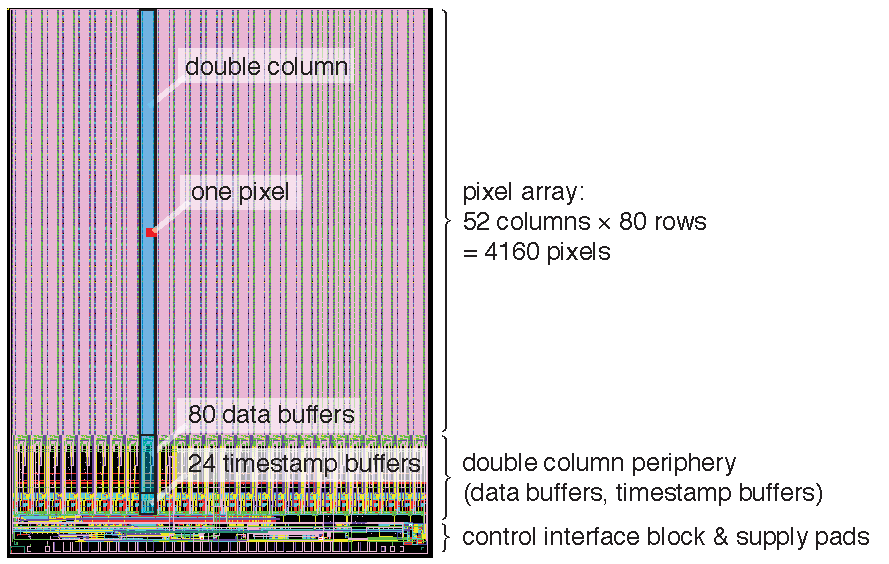
\includegraphics[width=.9\textwidth]{img/ROCimage.pdf}
	\end{center}
	\caption{Pixel chip arrangement. The image shows the full layout of a pixel chip. Highlighted are the areas of a single pixel, double column, the data buffers and the timestamp buffers. The periphery and the supply pads are in charge to handle trigger information, buffer data of recent pixel data and handle the communication with the outer world.}
	\label{fig:ROCimage}
\end{figure}

A \gls{PUC} is to a large extent an autonomously operating entity. The charge sensitive amplifier gets its input either from the attached sensor via a bump-pad or a special calibration mechanism (described later in this document). The amplifier output is passed through a signal shaper into a sample-and-hold circuit and into a charge discriminator. The latter is made of a voltage comparator with a programmable threshold voltage. Most of the time, the \gls{PUC} is in the \emph{sample} state. If the charge discriminator senses a signal above threshold, the sample-and-hold switches to \emph{hold} and signals the periphery a hit via a line shared by all \gls{PUC} in the \gls{DC}. For a properly calibrated \gls{PUC} this happens when the sensor gets hit by a charged particle. For others it may happen by noise. The measured charge is a function of the observed pulse height at the input of the amplifier. This function is mostly linear and saturates for high amounts of charge.

Every \gls{DC} has its own periphery. If a hit gets detected, the \emph{column drain} mechanism starts its work. It doesn't matter how many hits were detected in the \gls{DC} as this signal acts as a global logical OR of all \gls{PUC}. The first step of the column drain is to record the time stamp, which is the momentary content of an 8-bit counter. That counter gets increased with every clock cycle, hence there is a maximum trigger latency of $255\times25\,\text{ns}=6.375\,\mu\text{s}$, given by the size of this counter. This allows to match the hit to a certain LHC bunch crossing, which runs at the same 40\,MHz clock as the \gls{ROC}. For temporary data keeping, a token mechanism passes through the \gls{DC} and copies the charge of the individual sample-and-hold circuits down to the data buffers in the periphery, an analog process. Digitization happens later.

Up to this stage, no triggers were involved. Every \gls{PUC} and \gls{DC} works by itself, time stamps get assigned, charge gets copied down into the periphery. If no trigger signal reaches the chip, old data gets overwritten in the periphery. Hits in subsequent clock cycles can be correctly assigned to a certain time stamp as long as not more than two column drain operations are pending. If there are more than one working column drain and two pending ones, hits start to get assigned to the wrong time stamp, a possible source of inefficiency. As one \gls{DC} has 160\,\gls{PUC}, quite a fair amount of particle flux is needed to hit this limit\footnote{This becomes a problem in the innermost BPix layer. As os writing this text, a special chip, capable of handling higher fluxes, is under development for this case.}.

Now add triggers. There is a second 8-bit counter in the periphery that runs with a programmabke offset to the primary one. This offset is controlled by the so-called \emph{WBC} register. With a delay of exactly that number of clock cycles or bucnh crossings, a trigger signal must appear on the corresponding chip input. If this is the case, all \gls{DC} having hits matching this bunch crossing stop their normal operation and are put on halt. This is to preserve the data and protect it from accidential overwriting by still working \gls{DC}. The data gets transferred to the central readout buffer. The charge is transferred to the 8-bit ADC (one per \gls{ROC}) to digitize it. For every hit, the column number (6\,bits), the row number (9\,bits) and the pulse-height (8\,bits) get stored. One hit requires 23\,bits of storage. The readout buffer is designed as a FIFO with simultaneous read and write capability, and has a storage capacity of 64 such 23\,bit-words.

So far, nothing has been said about tokens. Sensor modules are made up of several \gls{ROC}, which are electrically grouped together. For example, on layer 4 BPix modules and all FPix modules, 8\,\gls{ROC} make up a readout group. The token is a signal to control the readout of \gls{ROC} in one such group. Assume several \gls{ROC} received hits in the same bunch crossing. All received a trigger signal at the same time, so the data has been transferred to the individual ROCs periphery and are now ready to be read out. With only a short delay after the trigger signal was received, the \gls{TBM} chip on the module sends out a token to the first chip in that group\footnote{The \gls{TBM} has more functionality than just passing a trigger from the CMS DAQ system to the \gls{ROC} and sending out a token. But this is beyond the scope of this document.}. All the data of that chip gets sent to the output data line. After all data has been sent, the \gls{ROC} sends a token to the next \gls{ROC}, which will immediately start its data transfer. This goes on until the last \gls{ROC} in that daisy-chain and the readout is finished. Upon sending the token to the next \gls{ROC}, all the \gls{DC} get re-enabled again and the chip is ready for further data taking. This design allows to use one data channel for a group of \gls{ROC}.

A word on calibration: Known amounts of charge can be injected from a circuit into individual \gls{PUC}. This allows to calibrate the amplifiers. But be aware: The voltage to control this charge is generated at one spot for the whole \gls{ROC}. While it is possible to transfer it to many \gls{PUC}, there is a risk to overload that circuit. Therefore do not use this mechanism to provide calibration pulses to more than a handful of pixels at the same time. The thresholds of the comparators are set with a voltage common to all \gls{PUC} in a \gls{ROC}. To adjust for pixel-to-pixel variations, every \gls{PUC} has its own 4-bit DAC to fine-tune the comparator.

